\begin{enumerate}

  \item {\bf Boundary-Value Problems}\label{s:heat1D}

    The heat equation on the other hand is a boundary value problem. Here we
    represent the pipe without time such that $T = f(x)$ instead of
    time. 

    \begin{equation} 
      \frac{d^2 T}{d x^2} - h'(T-T_a) = 0
    \end{equation}
    
    Thus the difference between boundary value problems and initial
    condition problems is really the independent variable. To solve
    this we set $T = Ce^{sx}+T_a$. We substitute this equation into 
    the equation above and obtain the characteristic equation and
    solve for s = $\pm\sqrt{h'}$. This yields the analytical solution
    $T(x) = A e^{\sqrt{h'}x} + B e^{-\sqrt{h'}x} + T_a$. Again the boundary
    conditions can be used to solve for A and B. For example, $T(x=0)
    = 40$ and $T(x=L) = 200$. Note that solving for A and B yields a
    system of equations. The solution to A and B has been left for the
    reader. 

    Now, in order to solve this equation numerically you must replace
    all derivatives with finite difference approximations. Below is a
    center first order approximation of the second derivative.

    \begin{equation}
      \frac{T_{i+1} - 2T_i + T_{i-1}}{\Delta x^2} - h'(T_i-T_a) = 0
    \end{equation}

    or

    \begin{equation}
      -T_{i-1} + (2+h'\Delta x^2)T_i - T_{i+1} = h'\Delta x^2 T_a
    \end{equation}

    If the rod is discretized into 6 beads ($\Delta x = 2$ and L = 10
    m) such that $T(0) = T_0 = 40$ and $T(L) = T_5 = 200$, letting
    h'=0.01 and $T_a = 20$ yields a system of equations

    \begin{equation}
      \begin{bmatrix} 2.04 & -1 & 0 & 0 \\ -1 & 2.04 & -1 & 0 \\ 0 &
        -1 & 2.04 & -1 \\ 0 & 0 & -1 &
        2.04\end{bmatrix} \begin{Bmatrix} T_1 \\ T_2 \\ T_3
          \\ T_4 \end{Bmatrix} = \begin{Bmatrix} 40.8 \\ 0.8 \\ 0.8
          \\ 200.8 \end{Bmatrix}
    \end{equation}

    which can be solved with any numerical solver. In this case $T = [
      65.970,93.778,124.538,159.480]$. Note, this can also
    be done using an iterative method. If the candidate equation is
    written such that
    
    \begin{equation}
      T_{i} = \frac{T_{i-1} + h'\Delta x^2 T_a + T_{i+1}}{2+h'\Delta x^2}
    \end{equation}

    The problem above evolves into a Simple Fixed Point Iteration
    Problem where the output is computed for every location $i$ along
    the rod and the solution is used to compute the next solution. The
    code required to implement the Simple Fixed Point Iteration
    technique is shown below.

    \begin{framed}
      x = 0:2:10;

      Tguess = 0*x;

      Tguess(1) = 20;

      Tguess(end) = 200;

      Ta = 20;

      hprime = 0.01;

      for iter = 1:100

      ~~~~~~for idx = 2:length(Tguess)-1

      ~~~~~~~~~~~~Tguess(idx) = (Tguess(idx-1) + hprime*delx{\textrm{\^}2}*Ta + Tguess(idx+1))/(2+hprime*delx{\textrm{\^}2});

      ~~~~~~end

      end
    \end{framed}

    The benefit of this code over solving the system using
    $A\vec{x}=B$ is that the number of beads can be arbitrarily
    increased without any change to the code. The solution to the code
    above can be plotted alongside the analytical solution and is
    shown in the equation below. Note that the solution below has 11
    beads rather than 6 beads. 

    \begin{figure}[H]
     \begin{center}
       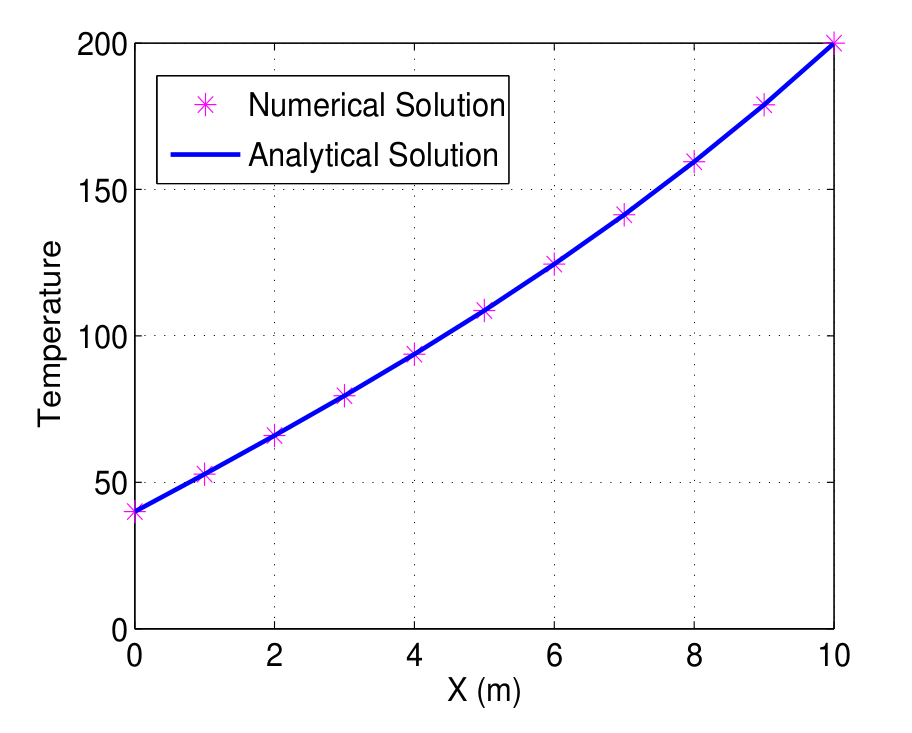
\includegraphics[height=0.4\textwidth,width=0.5\textwidth]{Graphics/Heat_Equation}
     \end{center}
   \end{figure}

\end{enumerate}
